\newcommand{\symactor}{\tikz[baseline=-0.1cm, scale=0.55, every node/.style={font=\tiny}]{\pic{actor={}};}}
\newcommand{\symuc}{\tikz[baseline=-0.1cm]\node[ellipse, draw, font=\scriptsize, inner sep=1.5pt]{Use Case};}
\newcommand{\symsys}{\tikz[baseline=-0.1cm]{\draw (0,0.3) rectangle (2,-0.3); \node[font=\tiny] at (1,0.15) {System};}}
\newcommand{\symline}{\tikz[baseline=-0.1cm]\draw (0,0) -- (2,0);}
\newcommand{\symarrow}[1]{\tikz[baseline=-0.1cm]{\draw[dashed, -{Stealth[length=1.6mm]}] (0,0) -- (2,0); \node[font=\tiny, above] at (1,0) {#1};}}
\newcommand{\symgen}{\tikz[baseline=-0.1cm]\draw[-{Triangle[open, length=2.2mm, width=2.2mm]}] (0,0) -- (2,0);}
\newcommand{\symreal}{\tikz[baseline=-0.1cm]\draw[dashed, -{Triangle[open, length=2.2mm, width=2.2mm]}] (0,0) -- (2,0);}
\newcommand{\symdep}{\tikz[baseline=-0.1cm]\draw[dashed, -{Stealth[length=1.6mm]}] (0,0) -- (2,0);}
\newcommand{\symagg}{\tikz[baseline=-0.1cm]\draw[{Diamond[open, length=2.6mm, width=1.8mm]}-] (0,0) -- (2,0);}
\newcommand{\symcomp}{\tikz[baseline=-0.1cm]\draw[{Diamond[length=2.6mm, width=1.8mm]}-] (0,0) -- (2,0);}
\newcommand{\symsync}{\tikz[baseline=-0.1cm]\draw[-{Triangle[length=2mm, width=2mm]}] (0,0) -- (2,0);}
\newcommand{\symasync}{\tikz[baseline=-0.1cm]\draw[-{Stealth[open, length=2mm]}] (0,0) -- (2,0);}
\newcommand{\symreply}{\tikz[baseline=-0.1cm]\draw[dashed, -{Stealth[open, length=2mm]}] (2,0) -- (0,0);}
\newcommand{\symlifeline}{\tikz[baseline=-0.25cm]{\node[draw, font=\tiny, inner sep=2pt] (o) at (0,0) {:Object}; \draw[dashed] (o.south) -- ++(0,-0.4);}}
\newcommand{\syminit}{\tikz[baseline=-0.1cm]\fill (0,0) circle (1.4mm);}
\newcommand{\symfinal}{\tikz[baseline=-0.1cm]{\draw (0,0) circle (1.8mm); \fill (0,0) circle (1.1mm);}}
\newcommand{\symstate}[1]{\tikz[baseline=-0.1cm]\node[draw, rounded corners=4pt, font=\scriptsize, minimum width=1.8cm]{#1};}
\newcommand{\symtrans}{\tikz[baseline=-0.1cm]{\draw[-{Stealth[length=1.6mm]}] (0,0) -- (2,0); \node[font=\tiny, above] at (1,0) {event [guard] / action};}}
\newcommand{\symdecision}{\tikz[baseline=-0.1cm]\node[diamond, draw, minimum size=4mm, inner sep=0pt]{};}
\newcommand{\symfork}{\tikz[baseline=-0.1cm]\fill (0,-0.05) rectangle (2,0.05);}
\newcommand{\symflow}{\tikz[baseline=-0.1cm]\draw[-{Stealth[length=1.6mm]}] (0,0) -- (2,0);}
\newcommand{\sympkg}{\tikz[baseline=-0.1cm]{\draw (0,0.25) rectangle (0.6,0.4); \draw (0,0.25) rectangle (1.6,-0.3); \node[font=\tiny] at (0.8,-0.03) {package};}}
\newcommand{\symcompnt}{\tikz[baseline=-0.1cm]{\node[draw, font=\tiny, align=center, inner sep=2pt] {<{}<component>{}>\\Name};}}
\newcommand{\symball}{\tikz[baseline=-0.1cm]{\draw (0,0) -- (0.9,0); \draw[fill=white] (1.05,0) circle (1.5mm);}}
\newcommand{\symnode}{\tikz[baseline=-0.1cm]{\draw (0,0.25) rectangle (1.4,-0.35); \draw (0,0.25) -- (0.2,0.42) -- (1.6,0.42) -- (1.6,-0.18) -- (1.4,-0.35); \draw (1.4,0.25) -- (1.6,0.42); \node[font=\tiny] at (0.7,-0.05) {Node};}}

\newcommand{\ucscenario}[7]{%
\needspace{7\baselineskip}
\begin{xltabular}{\textwidth}{|p{3.4cm}|Y|}
\caption{Use case scenario: #2}\\
\hline
\textbf{Use Case ID} & #1 \\ \hline
\textbf{Use Case Name} & #2 \\ \hline
\textbf{Actors} & #3 \\ \hline
\textbf{Precondition} & #4 \\ \hline
\textbf{Main Flow} & #5 \\ \hline
\textbf{Alternative Flow} & #6 \\ \hline
\textbf{Postcondition} & #7 \\ \hline
\end{xltabular}}

\newsection{UML Modelling}{sec:uml}

The Unified Modeling Language (UML) is the standard visual language for specifying, constructing and documenting the parts of an object-oriented system [1], [2]. This section models FacultyDesk with the main UML diagrams. For each diagram it gives the theory and notation, the diagram for the project, an explanation, supporting tables and a short conclusion. All class, method, state and attribute names in the diagrams are taken from the project's source code.

\needspace{7\baselineskip}
\begin{xltabular}{\textwidth}{|p{4.6cm}|p{3cm}|Y|}
\caption{UML diagrams presented in this report}\\
\hline
\textbf{Diagram} & \textbf{Kind} & \textbf{What it shows for FacultyDesk} \\ \hline
Use case diagram & Behavioural & Actors and the services the system gives them \\ \hline
Class diagram & Structural & Domain classes, attributes, operations and relations \\ \hline
Sequence diagram & Interaction & Time order of messages in three key flows \\ \hline
Collaboration diagram & Interaction & Objects and numbered messages when a circular is confirmed \\ \hline
Statechart diagram & Behavioural & Life cycles of Circular, ScheduledNotification and TimetableUpload \\ \hline
Activity diagram & Behavioural & Workflow of timetable ingestion across three swimlanes \\ \hline
Package diagram & Structural & Code packages and their dependencies \\ \hline
Component diagram & Structural & Runtime components and the interfaces between them \\ \hline
Deployment diagram & Structural & Containers on the department server and the network links \\ \hline
Entity--relationship diagram & Data model & Database tables, keys and relations \\ \hline
\end{xltabular}

\subsection{Use Case Diagram}

\theory{Theory}
A use case diagram is a behavioural UML diagram that gives a high-level picture of \emph{what} a system offers to its users, without describing \emph{how} each function is built. It contains the system boundary, the actors outside it, the use cases inside it, and the relationships among them.
\begin{itemize}
  \item \textbf{Actor:} an external role that interacts with the system to reach a goal. A \emph{primary actor} starts the use case; a \emph{supporting actor} helps the system deliver it. An actor may be a person or another system, such as a scheduler.
  \item \textbf{Use case:} a unit of functionality that gives an observable result of value to an actor, named with a verb phrase such as ``Upload timetable''.
  \item \textbf{System boundary:} a rectangle that encloses the use cases and defines the scope.
\end{itemize}

\theory{Use Case Notation}
\needspace{7\baselineskip}
\begin{xltabular}{\textwidth}{|p{3cm}|>{\centering\arraybackslash}p{3.3cm}|Y|}
\caption{Use case diagram notation}\\
\hline
\textbf{Element} & \textbf{Symbol} & \textbf{Meaning} \\ \hline
Actor & \symactor & A role played by a user or an external system. \\ \hline
Use case & \symuc & A function the system performs for an actor. \\ \hline
System boundary & \symsys & Encloses the use cases and defines the scope. \\ \hline
Association & \symline & The actor takes part in the use case. \\ \hline
Include & \symarrow{<{}<include>{}>} & The base use case always uses the included one. \\ \hline
Extend & \symarrow{<{}<extend>{}>} & Optional behaviour added to a base use case under a condition. \\ \hline
Generalization & \symgen & The child is a specialised form of the parent. \\ \hline
\end{xltabular}

\begin{figure}[!htbp]
  \centering
  \resizebox{\textwidth}{!}{\begin{tikzpicture}[
    uc/.style={ellipse, draw, semithick, fill=ucfill, minimum width=4.1cm, minimum height=1.05cm, align=center, font=\footnotesize, inner sep=1pt},
    assoc/.style={semithick},
    rel/.style={-{Stealth[length=2.2mm]}, dashed, semithick},
    lbl/.style={font=\scriptsize\itshape, fill=white, inner sep=1pt}
  ]
  \draw[semithick, rounded corners=3pt, fill=sysfill] (2.55,-0.4) rectangle (13.75,19.1);
  \node[font=\bfseries] at (8.15,18.7) {FacultyDesk};

  \node[uc] (login) at (5.0,17.6) {Log in};
  \node[uc] (terms) at (5.0,16.1) {Manage terms\\and holidays};
  \node[uc] (dir) at (5.0,14.6) {Manage faculty\\directory};
  \node[uc] (uptt) at (5.0,13.1) {Upload timetable};
  \node[uc] (conftt) at (5.0,11.6) {Confirm timetable};
  \node[uc] (review) at (5.0,10.1) {Review circular};
  \node[uc] (assign) at (5.0,8.6) {Assign department\\tasks};
  \node[uc] (upcirc) at (5.0,7.1) {Upload circular};
  \node[uc] (cal) at (5.0,5.6) {View personal\\calendar};
  \node[uc] (tasks) at (5.0,4.1) {Manage own tasks};
  \node[uc] (prefs) at (5.0,2.6) {Set reminder rules\\and quiet hours};
  \node[uc] (ics) at (5.0,1.1) {Subscribe to\\ICS feed};

  \node[uc] (resolve) at (11.2,13.1) {Resolve faculty\\initials};
  \node[uc] (gen) at (11.2,11.6) {Generate weekly\\class events};
  \node[uc] (ocr) at (11.2,7.1) {Extract meeting\\fields by OCR};
  \node[uc] (free) at (11.2,5.6) {Find common\\free slots};
  \node[uc] (send) at (11.2,3.6) {Send reminders};
  \node[uc] (esc) at (11.2,2.2) {Escalate overdue\\tasks};
  \node[uc] (backup) at (11.2,0.8) {Back up\\database};

  \pic at (0.6,15.3) {actor={Admin}};
  \pic at (0.6,9.9) {actor={HOD}};
  \pic at (0.6,3.4) {actor={Faculty}};
  \pic at (15.6,2.4) {actor={Scheduler}};

  \coordinate (adm) at (1.05,15.75);
  \coordinate (hod) at (1.05,10.35);
  \coordinate (fac) at (1.05,3.85);
  \coordinate (sch) at (15.15,2.85);

  \foreach \u in {login,terms,dir,uptt} \draw[assoc] (adm) -- (\u.west);
  \foreach \u in {login,dir,uptt,conftt,review,assign,upcirc,cal} \draw[assoc] (hod) -- (\u.west);
  \foreach \u in {login,upcirc,cal,tasks,prefs,ics} \draw[assoc] (fac) -- (\u.west);
  \foreach \u in {send,esc,backup} \draw[assoc] (sch) -- (\u.east);

  \draw[rel] (uptt) -- node[lbl, above] {\guill{include}} (resolve);
  \draw[rel] (conftt) -- node[lbl, above] {\guill{include}} (gen);
  \draw[rel] (upcirc) -- node[lbl, above] {\guill{include}} (ocr);
  \draw[rel] (review.east) -- (7.9,10.1) -- node[lbl, right] {\guill{extend}} (7.9,7.6) -- (upcirc.25);
  \draw[rel] (free) -- node[lbl, above] {\guill{extend}} (cal);
\end{tikzpicture}
}
  \caption{FacultyDesk use case diagram}
  \label{fig:usecase}
\end{figure}

\head{Explanation}
\begin{itemize}
  \item \textbf{Actors:} \emph{Admin} manages terms, holidays and the faculty directory. \emph{HOD} uploads and confirms timetables, reviews circulars and assigns tasks. \emph{Faculty} upload circulars, view their calendar, manage tasks, set reminder preferences and subscribe to the ICS feed. \emph{Scheduler} is the background job runner (Celery Beat), a non-human actor.
  \item \textbf{Upload timetable} \guill{include} \textbf{Resolve faculty initials}, because a timetable can never be stored without knowing which teacher each cell refers to.
  \item \textbf{Confirm timetable} \guill{include} \textbf{Generate weekly class events}, because confirmation always creates the classes.
  \item \textbf{Upload circular} \guill{include} \textbf{Extract meeting fields by OCR}, because every uploaded circular is read.
  \item \textbf{Review circular} \guill{extend} \textbf{Upload circular}: review is needed only when the extraction fails the confidence gate.
  \item \textbf{Find common free slots} \guill{extend} \textbf{View personal calendar}: it is an optional step when planning a meeting.
  \item The Scheduler sends reminders, escalates overdue tasks and backs up the database without any human action.
\end{itemize}

\head{Actors and Use Cases Identified}
\needspace{7\baselineskip}
\begin{xltabular}{\textwidth}{|p{2.4cm}|p{2.6cm}|Y|}
\caption{Actors and use cases}\\
\hline
\textbf{Actor} & \textbf{Type} & \textbf{Use cases} \\ \hline
Admin & Primary & Log in, Manage terms and holidays, Manage faculty directory, Upload timetable \\ \hline
HOD & Primary & Log in, Manage faculty directory, Upload timetable, Confirm timetable, Review circular, Assign department tasks, Upload circular, View personal calendar \\ \hline
Faculty & Primary & Log in, Upload circular, View personal calendar, Manage own tasks, Set reminder rules and quiet hours, Subscribe to ICS feed \\ \hline
Scheduler & Supporting (system) & Send reminders, Escalate overdue tasks, Back up database \\ \hline
\end{xltabular}

\ucscenario{UC-01}{Upload and Confirm Timetable}{HOD (primary)}{HOD is logged in; the academic term exists; faculty profiles with initials exist in the department.}{1. HOD selects the term and uploads the timetable file (xlsx, csv or pdf, at most 15 MB).\newline 2. System checks the file type from its first bytes, stores it and starts parsing.\newline 3. System parses the grid, expands merged period cells and resolves each initials token (\emph{include: Resolve faculty initials}).\newline 4. System shows the preview slots and any unresolved tokens.\newline 5. HOD confirms the preview.\newline 6. System saves courses, sections, rooms and slots, and generates the weekly class events (\emph{include: Generate weekly class events}).}{2a. Unsupported file or scanned PDF without text: the upload is rejected with guidance.\newline 4a. Some initials are unresolved or ambiguous: HOD adds an alias in the directory and uploads again.}{Every teacher named in the timetable sees the term's classes on the calendar, without holidays, with reminders planned.}

\ucscenario{UC-02}{Upload and Confirm Meeting Circular}{Faculty or HOD (upload), HOD (review)}{User is logged in; department faculty have initials and aliases.}{1. User uploads a photo, scan or PDF of the circular.\newline 2. System stores it and replies at once; a worker processes it.\newline 3. System reads the text (PDF text layer, or image clean-up and Tesseract OCR) (\emph{include: Extract meeting fields by OCR}).\newline 4. System extracts date, time, venue, title, agenda and attendees.\newline 5. The circular fails the gate and enters the review queue (\emph{extend: Review circular}).\newline 6. HOD corrects any field and confirms.\newline 7. System creates a MEETING event for every attendee and plans their reminders.}{3a. File or OCR error: circular becomes FAILED and can be processed again.\newline 5a. All fields pass the gate and the department allows automatic confirmation: the meeting is created without review.\newline 6a. HOD rejects the circular: it becomes REJECTED and no event is created.}{Each named attendee sees the meeting and receives reminders at their chosen lead times.}

\ucscenario{UC-03}{Send Reminders}{Scheduler (primary), Faculty (receiver)}{Pending reminders exist with a fire time in the past; the user has an e-mail address or a push subscription.}{1. Every 30 seconds the Scheduler starts the dispatch job.\newline 2. System claims up to 100 due reminders, locking them so no other worker takes them.\newline 3. For each reminder, the system builds the message from the event or task.\newline 4. The reminder is sent by e-mail or web push and marked SENT.}{3a. The task is already completed: the reminder is cancelled.\newline 4a. Sending fails: the reminder is retried later, up to five attempts, then marked FAILED.}{Each reminder is delivered at most once; the Admin can see delivery counts and failures.}

\ucscenario{UC-04}{Assign and Complete Documentation Task}{HOD (assign), Faculty (complete)}{HOD and faculty accounts exist; task templates are seeded.}{1. HOD picks a template (for example IA marks upload) or writes a task, sets a deadline and importance.\newline 2. HOD assigns it to one teacher, a group or the whole department.\newline 3. System creates one task per assignee, a DEADLINE event on each calendar, and alerts at 72 h, 24 h and 2 h before the deadline.\newline 4. Faculty see the task ranked by priority and mark it complete.\newline 5. System cancels the remaining alerts and updates the HOD dashboard.}{4a. Deadline passes: daily overdue alerts start and the HOD receives an escalation summary.\newline 5a. Faculty reopen the task: future alerts are scheduled again.}{The HOD dashboard shows the completion rate and overdue count per teacher.}

\head{Conclusion}
The use case diagram captures every service of FacultyDesk and who uses it. The \guill{include} relation models mandatory steps such as initials resolution and OCR, and \guill{extend} models optional steps such as review and free-slot finding.

\subsection{Class Diagram}

\theory{Theory}
A class diagram is a structural UML diagram that shows the classes of a system, their attributes and operations, and the relationships between them. It is the main diagram of object-oriented design and maps directly to code. A class is drawn as a rectangle with three compartments: name, attributes and operations. Visibility is shown with \textbf{+} public, \textbf{--} private, \textbf{\#} protected and \textbf{\textasciitilde} package.

\theory{Relationships Between Classes}
\needspace{7\baselineskip}
\begin{xltabular}{\textwidth}{|p{3cm}|>{\centering\arraybackslash}p{3cm}|Y|}
\caption{Class relationship notation}\\
\hline
\textbf{Relationship} & \textbf{Symbol} & \textbf{Example in FacultyDesk} \\ \hline
Association & \symline & FacultyProfile belongs to a Department. \\ \hline
Aggregation & \symagg & CompositeNotifier has an EmailNotifier and a WebPushNotifier. \\ \hline
Composition & \symcomp & Event owns its EventAttendees; AcademicTerm owns its Holidays. \\ \hline
Generalization & \symgen & XlsxTimetableParser is a TimetableParser. \\ \hline
Realization & \symreal & SystemClock implements the Clock protocol. \\ \hline
Dependency & \symdep & A Circular creates an Event when confirmed. \\ \hline
\end{xltabular}

\theory{Multiplicity}
\begin{table}[H]
\centering
\begin{tabular}{|p{2.6cm}|p{6.6cm}|}
\hline
\textbf{Notation} & \textbf{Meaning} \\ \hline
1 & Exactly one \\ \hline
0..1 & Zero or one \\ \hline
* or 0..* & Zero or more \\ \hline
1..* & One or more \\ \hline
\end{tabular}
\caption{Multiplicity notation}
\end{table}

\begin{figure}[!htbp]
  \centering
  \resizebox{\textwidth}{!}{\begin{tikzpicture}[
    assoc/.style={semithick},
    comp/.style={semithick, {Diamond[length=3mm, width=2mm, fill=black]}-},
    dep/.style={semithick, dashed, -{Stealth[length=2.2mm]}},
    m/.style={font=\scriptsize, inner sep=1.5pt},
    lbl/.style={font=\scriptsize\itshape, fill=white, inner sep=1pt}
  ]
  \umlclass{dept}{0,0}{Department}{
    + id : UUID\\
    + code : str\\
    + name : str}{}
  \umlclass{fp}{4.8,0}{FacultyProfile}{
    + id : UUID\\
    + full\_name : str\\
    + initials : Initials\\
    + aliases : tuple[str]\\
    + email : str\\
    + ics\_token : str}{}
  \umlclass{user}{9.6,0}{User}{
    + id : UUID\\
    + email : str\\
    + password\_hash : str\\
    + role : Role\\
    + is\_active : bool}{
    + quiet\_hours() : QuietHours}
  \umlclass{rule}{14.4,0}{ReminderRule}{
    + event\_kind : EventKind\\
    + offsets\_minutes : tuple[int]\\
    + channels : tuple[Channel]}{}

  \umlclass{term}{0,-5.4}{AcademicTerm}{
    + name : str\\
    + start\_date : date\\
    + end\_date : date\\
    + timezone : str}{}
  \umlclass{att}{4.8,-5.4}{EventAttendee}{
    + event\_id : UUID\\
    + faculty\_id : UUID\\
    + response : AttendeeResponse}{}
  \umlclass{event}{9.6,-5.4}{Event}{
    + kind : EventKind\\
    + title : str\\
    + start\_utc : datetime\\
    + end\_utc : datetime\\
    + location : str\\
    + source : EventSource}{
    + reschedule(start, end)\\
    + cancel(reason)\\
    + add\_attendee(faculty\_id)}
  \umlclass{task}{14.4,-5.4}{Task}{
    + title : str\\
    + deadline\_utc : datetime\\
    + importance : int [1..5]\\
    + category : TaskCategory\\
    + status : TaskStatus}{
    + update\_deadline(d)\\
    + change\_status(s)}

  \umlclass{hol}{0,-10.8}{Holiday}{
    + date : date\\
    + label : str}{}
  \umlclass{slot}{4.8,-10.8}{TimetableSlot}{
    + time\_slot : TimeSlot\\
    + course\_id : UUID\\
    + section\_id : UUID\\
    + room\_id : UUID\\
    + faculty\_id : UUID}{}
  \umlclass{circ}{9.6,-10.8}{Circular}{
    + file\_key : str\\
    + ocr\_text : str\\
    + extracted\_fields : dict\\
    + confidence : float\\
    + status : CircularStatus}{
    + start\_processing()\\
    + mark\_needs\_review(f, c)\\
    + confirm(f) / reject(r) / fail(r)}
  \umlclass{notif}{14.4,-10.8}{ScheduledNotification}{
    + channel : Channel\\
    + fire\_at\_utc : datetime\\
    + idempotency\_key : str\\
    + attempts : int\\
    + status : NotificationStatus}{
    + mark\_sending() / mark\_sent()\\
    + mark\_failed(e) / retry()\\
    + cancel()}

  \umlclass{upload}{4.8,-16.0}{TimetableUpload}{
    + file\_key : str\\
    + status : UploadStatus\\
    + parse\_report : dict}{
    + start\_parsing()\\
    + mark\_preview\_ready(r)\\
    + confirm() / fail(r)}

  \draw[assoc] (dept) -- node[m, above, pos=0.18] {1} node[m, above, pos=0.82] {*} node[lbl, below] {employs} (fp);
  \draw[assoc] (user) -- node[m, above, pos=0.18] {1} node[m, above, pos=0.82] {0..1} node[lbl, below] {has} (fp);
  \draw[assoc] (user) -- node[m, above, pos=0.18] {1} node[m, above, pos=0.82] {*} node[lbl, below] {owns} (rule);
  \draw[comp] (term) -- node[m, right, pos=0.15] {1} node[m, right, pos=0.85] {*} (hol);
  \draw[assoc] (fp) -- node[m, right, pos=0.15] {1} node[m, right, pos=0.85] {*} node[lbl, left] {attends} (att);
  \draw[comp] (event) -- node[m, above, pos=0.2] {1} node[m, above, pos=0.8] {*} (att);
  \draw[comp] (upload) -- node[m, right, pos=0.15] {1} node[m, right, pos=0.85] {*} (slot);
  \draw[assoc] (slot.west) -- ++(-0.45,0) |- node[lbl, pos=0.25, left] {teaches} node[m, above, pos=0.93] {1} ([yshift=-4mm]fp.west);
  \draw[dep] (slot.north east) -- node[lbl, sloped, above] {\guill{materialises}} (event.south west);
  \draw[dep] (circ) -- node[lbl, right] {\guill{creates}} (event);
  \draw[dep] (notif) -- node[lbl, sloped, above] {target} (event.south east);
  \draw[dep] (notif) -- node[lbl, right] {target} (task);
  \draw[assoc] (task.north) -- ++(0,0.5) -| node[m, right, pos=0.9] {1} node[lbl, pos=0.25, above] {assignee} ([xshift=9mm]user.south);
\end{tikzpicture}
}
  \caption{FacultyDesk domain class diagram}
  \label{fig:classdomain}
\end{figure}

\head{Classes Identified}
{\small
\begin{xltabular}{\textwidth}{|p{3.3cm}|Y|Y|}
\caption{Domain classes with attributes and operations}\\
\hline
\textbf{Class} & \textbf{Attributes} & \textbf{Operations / rules} \\ \hline
User & email, password\_hash, role, is\_active, quiet hours & quiet\_hours() \\ \hline
FacultyProfile & full\_name, initials, aliases, email, phone, ics\_token & initials must be 2--5 capital letters \\ \hline
Department & code, name & -- \\ \hline
AcademicTerm & name, start\_date, end\_date, timezone & owns Holidays \\ \hline
Holiday & date, label & -- \\ \hline
TimetableUpload & file\_key, status, parse\_report & start\_parsing(), mark\_preview\_ready(), confirm(), fail() \\ \hline
TimetableSlot & time\_slot, course, section, room, faculty & -- \\ \hline
Event & kind, title, start\_utc, end\_utc, location, source & reschedule(), cancel(), add\_attendee() \\ \hline
EventAttendee & event\_id, faculty\_id, response & -- \\ \hline
Circular & file\_key, ocr\_text, extracted\_fields, confidence, status & start\_processing(), mark\_needs\_review(), confirm(), reject(), fail() \\ \hline
ScheduledNotification & channel, fire\_at\_utc, idempotency\_key, attempts, status & mark\_sending(), mark\_sent(), mark\_failed(), retry(), cancel() \\ \hline
ReminderRule & event\_kind, offsets\_minutes, channels & offsets cannot be negative \\ \hline
Task & title, deadline\_utc, importance (1--5), category, status & update\_deadline(), change\_status() \\ \hline
\end{xltabular}}

\head{Relationships}
\begin{itemize}
  \item \textbf{FacultyProfile} is the central class: it belongs to a \textbf{Department}, is linked to one \textbf{User} account, teaches \textbf{TimetableSlot}s and attends \textbf{Event}s through \textbf{EventAttendee}.
  \item \textbf{Composition:} a \textbf{TimetableUpload} owns its slots, an \textbf{Event} owns its attendees, and an \textbf{AcademicTerm} owns its holidays; the parts have no meaning without the whole.
  \item \textbf{Event} is one class for classes, meetings and deadlines; its \texttt{kind} attribute tells them apart, so clash detection, reminders and the ICS feed treat them the same way.
  \item A confirmed \textbf{TimetableSlot} is \emph{materialised} into weekly CLASS events, and a confirmed \textbf{Circular} \emph{creates} one MEETING event.
  \item A \textbf{ScheduledNotification} targets an \textbf{Event} or a \textbf{Task}; a \textbf{Task} has one assignee \textbf{User}.
\end{itemize}

\head{Conclusion}
The class diagram shows that the business rules live in the classes themselves: each class validates its own data and controls its own status changes, which is the basis of the object-oriented design.

\subsection{Sequence Diagrams}

\theory{Theory}
A sequence diagram is an interaction diagram that shows how objects communicate by exchanging messages in time order. Time flows from top to bottom. Each participant has a lifeline; messages are arrows between lifelines; combined fragments such as \texttt{alt} (alternatives) and \texttt{loop} (repetition) group messages.

\theory{Sequence Diagram Notation}
\needspace{7\baselineskip}
\begin{xltabular}{\textwidth}{|p{3.2cm}|>{\centering\arraybackslash}p{3cm}|Y|}
\caption{Sequence diagram notation}\\
\hline
\textbf{Element} & \textbf{Symbol} & \textbf{Meaning} \\ \hline
Lifeline & \symlifeline & An object taking part in the interaction. \\ \hline
Synchronous message & \symsync & The sender waits for the reply. \\ \hline
Asynchronous message & \symasync & The sender continues without waiting. \\ \hline
Reply message & \symreply & Return of control or a value. \\ \hline
Self message & -- & A message an object sends to itself. \\ \hline
alt / loop fragment & -- & Alternative paths with guards / repeated messages. \\ \hline
\end{xltabular}

\begin{figure}[!htbp]
  \centering
  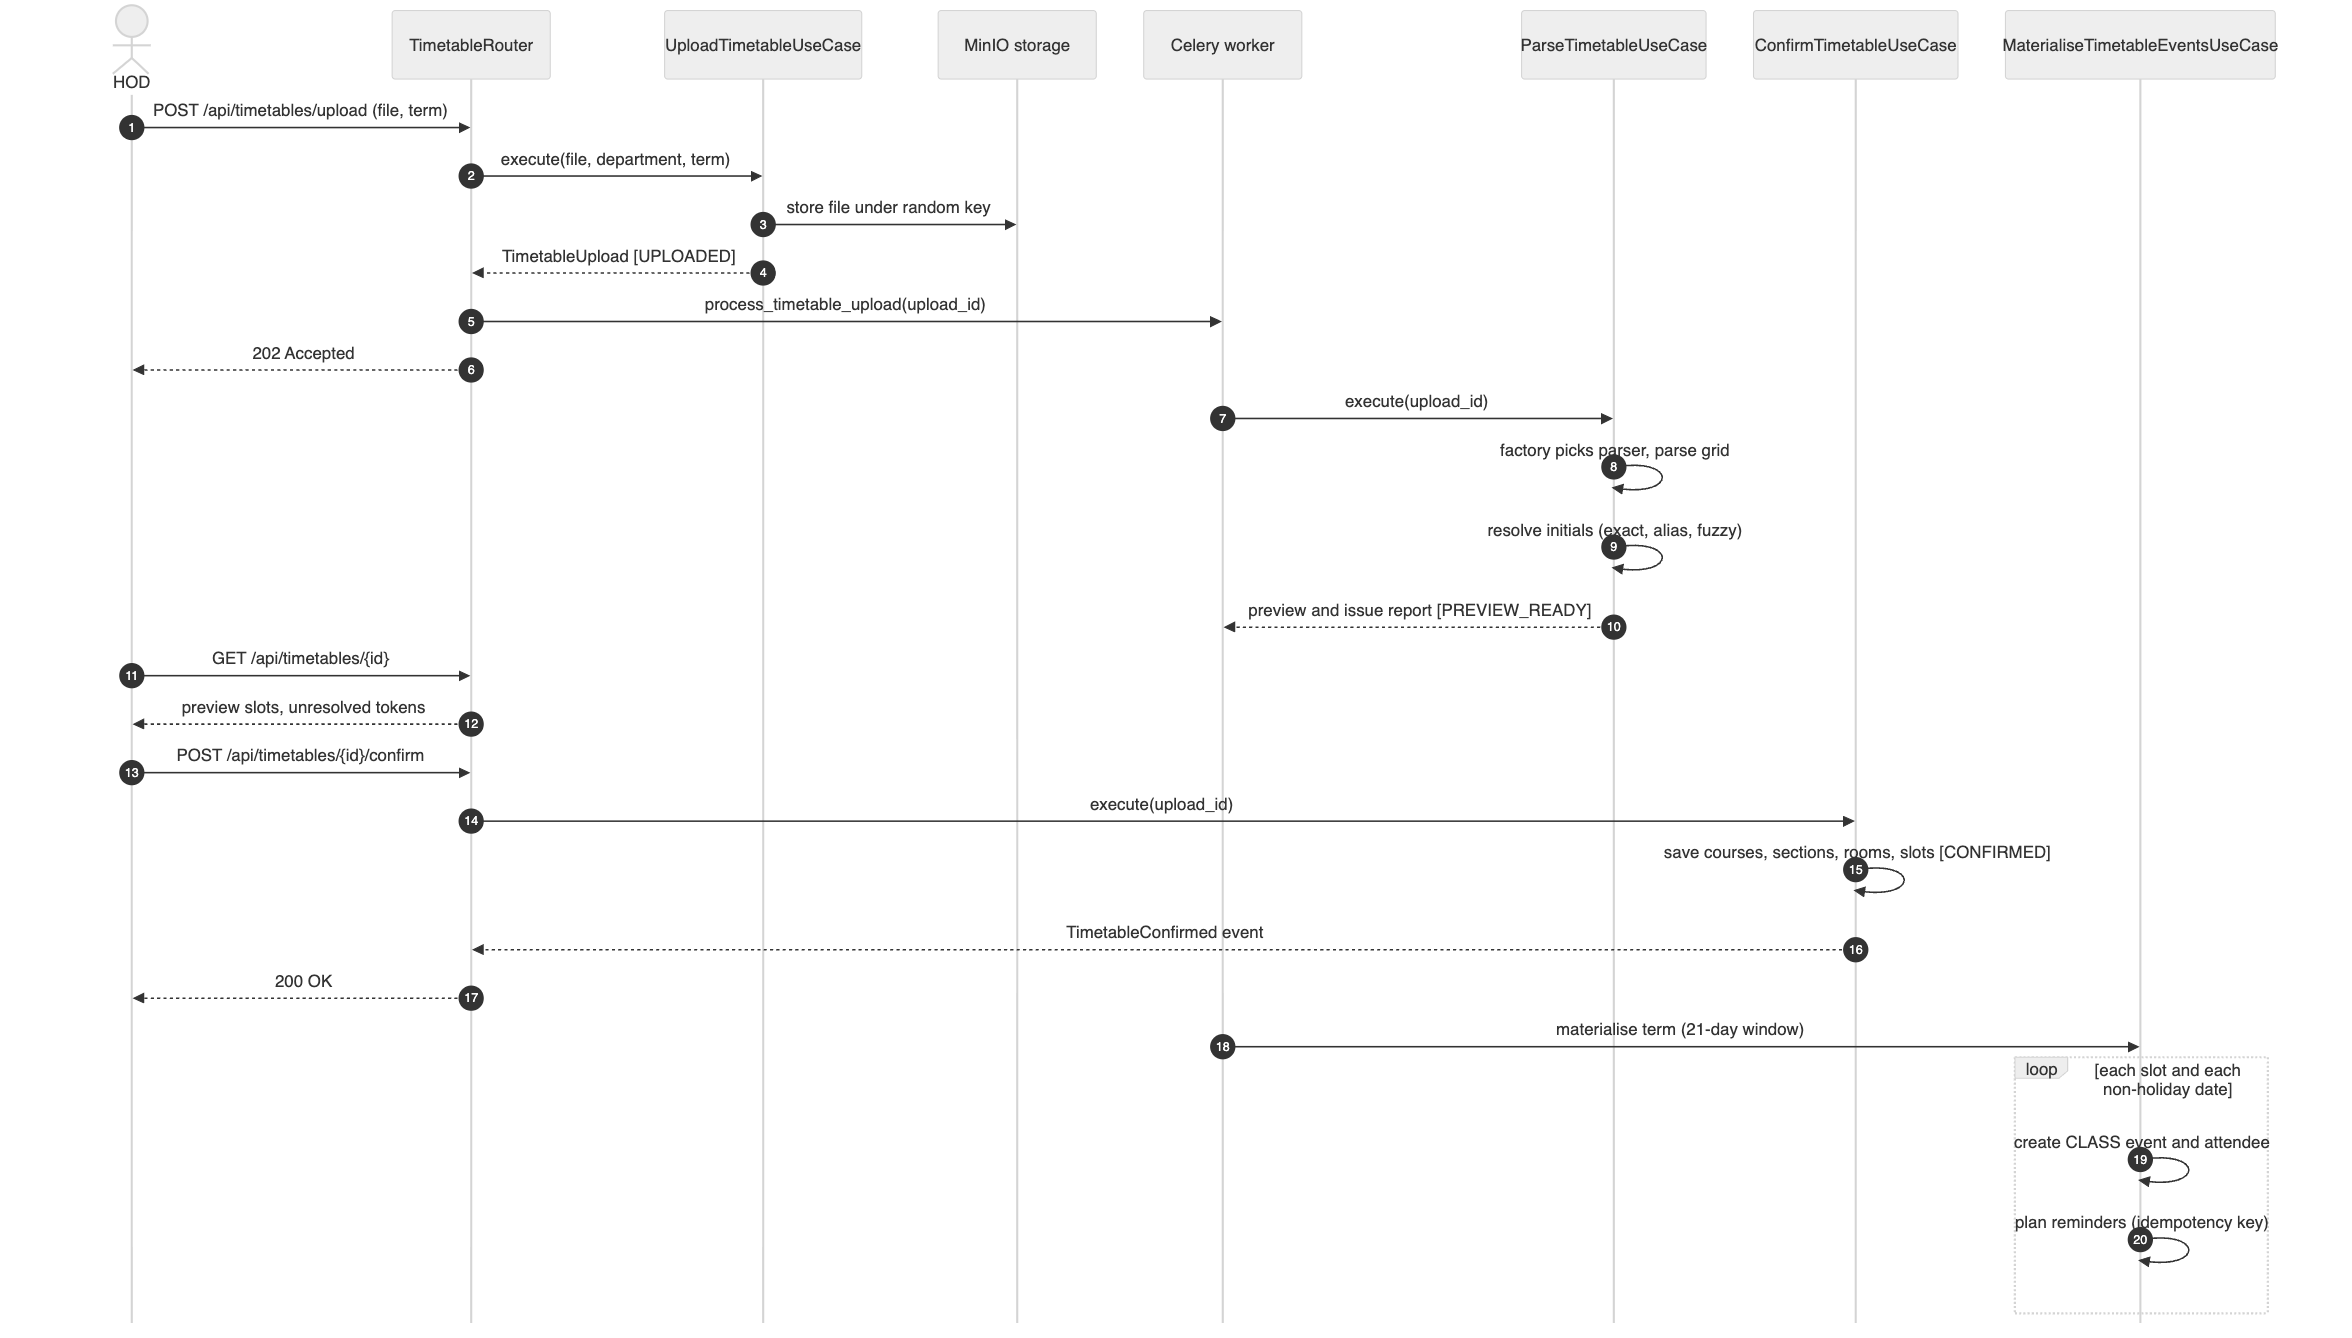
\includegraphics[width=\textwidth]{figures/seq_timetable.png}
  \caption{Sequence diagram: timetable upload and class generation}
  \label{fig:seqtt}
\end{figure}

\head{Explanation}
\begin{enumerate}
  \item The HOD uploads the file (1). The router passes it to \texttt{UploadTimetableUseCase}, which stores it and returns a \texttt{TimetableUpload} in state UPLOADED (2--4).
  \item The router hands parsing to a Celery worker and replies \texttt{202 Accepted} at once (5--6), so the web request stays short.
  \item The worker runs \texttt{ParseTimetableUseCase}: the factory picks the parser and the initials are resolved (7--10).
  \item The HOD reads the preview (11--12) and confirms (13). \texttt{ConfirmTimetableUseCase} saves the slots and raises a \texttt{TimetableConfirmed} event (14--17).
  \item The worker then expands each slot over the term in a \texttt{loop}, creating CLASS events and planning reminders (18--20).
\end{enumerate}

\begin{figure}[!htbp]
  \centering
  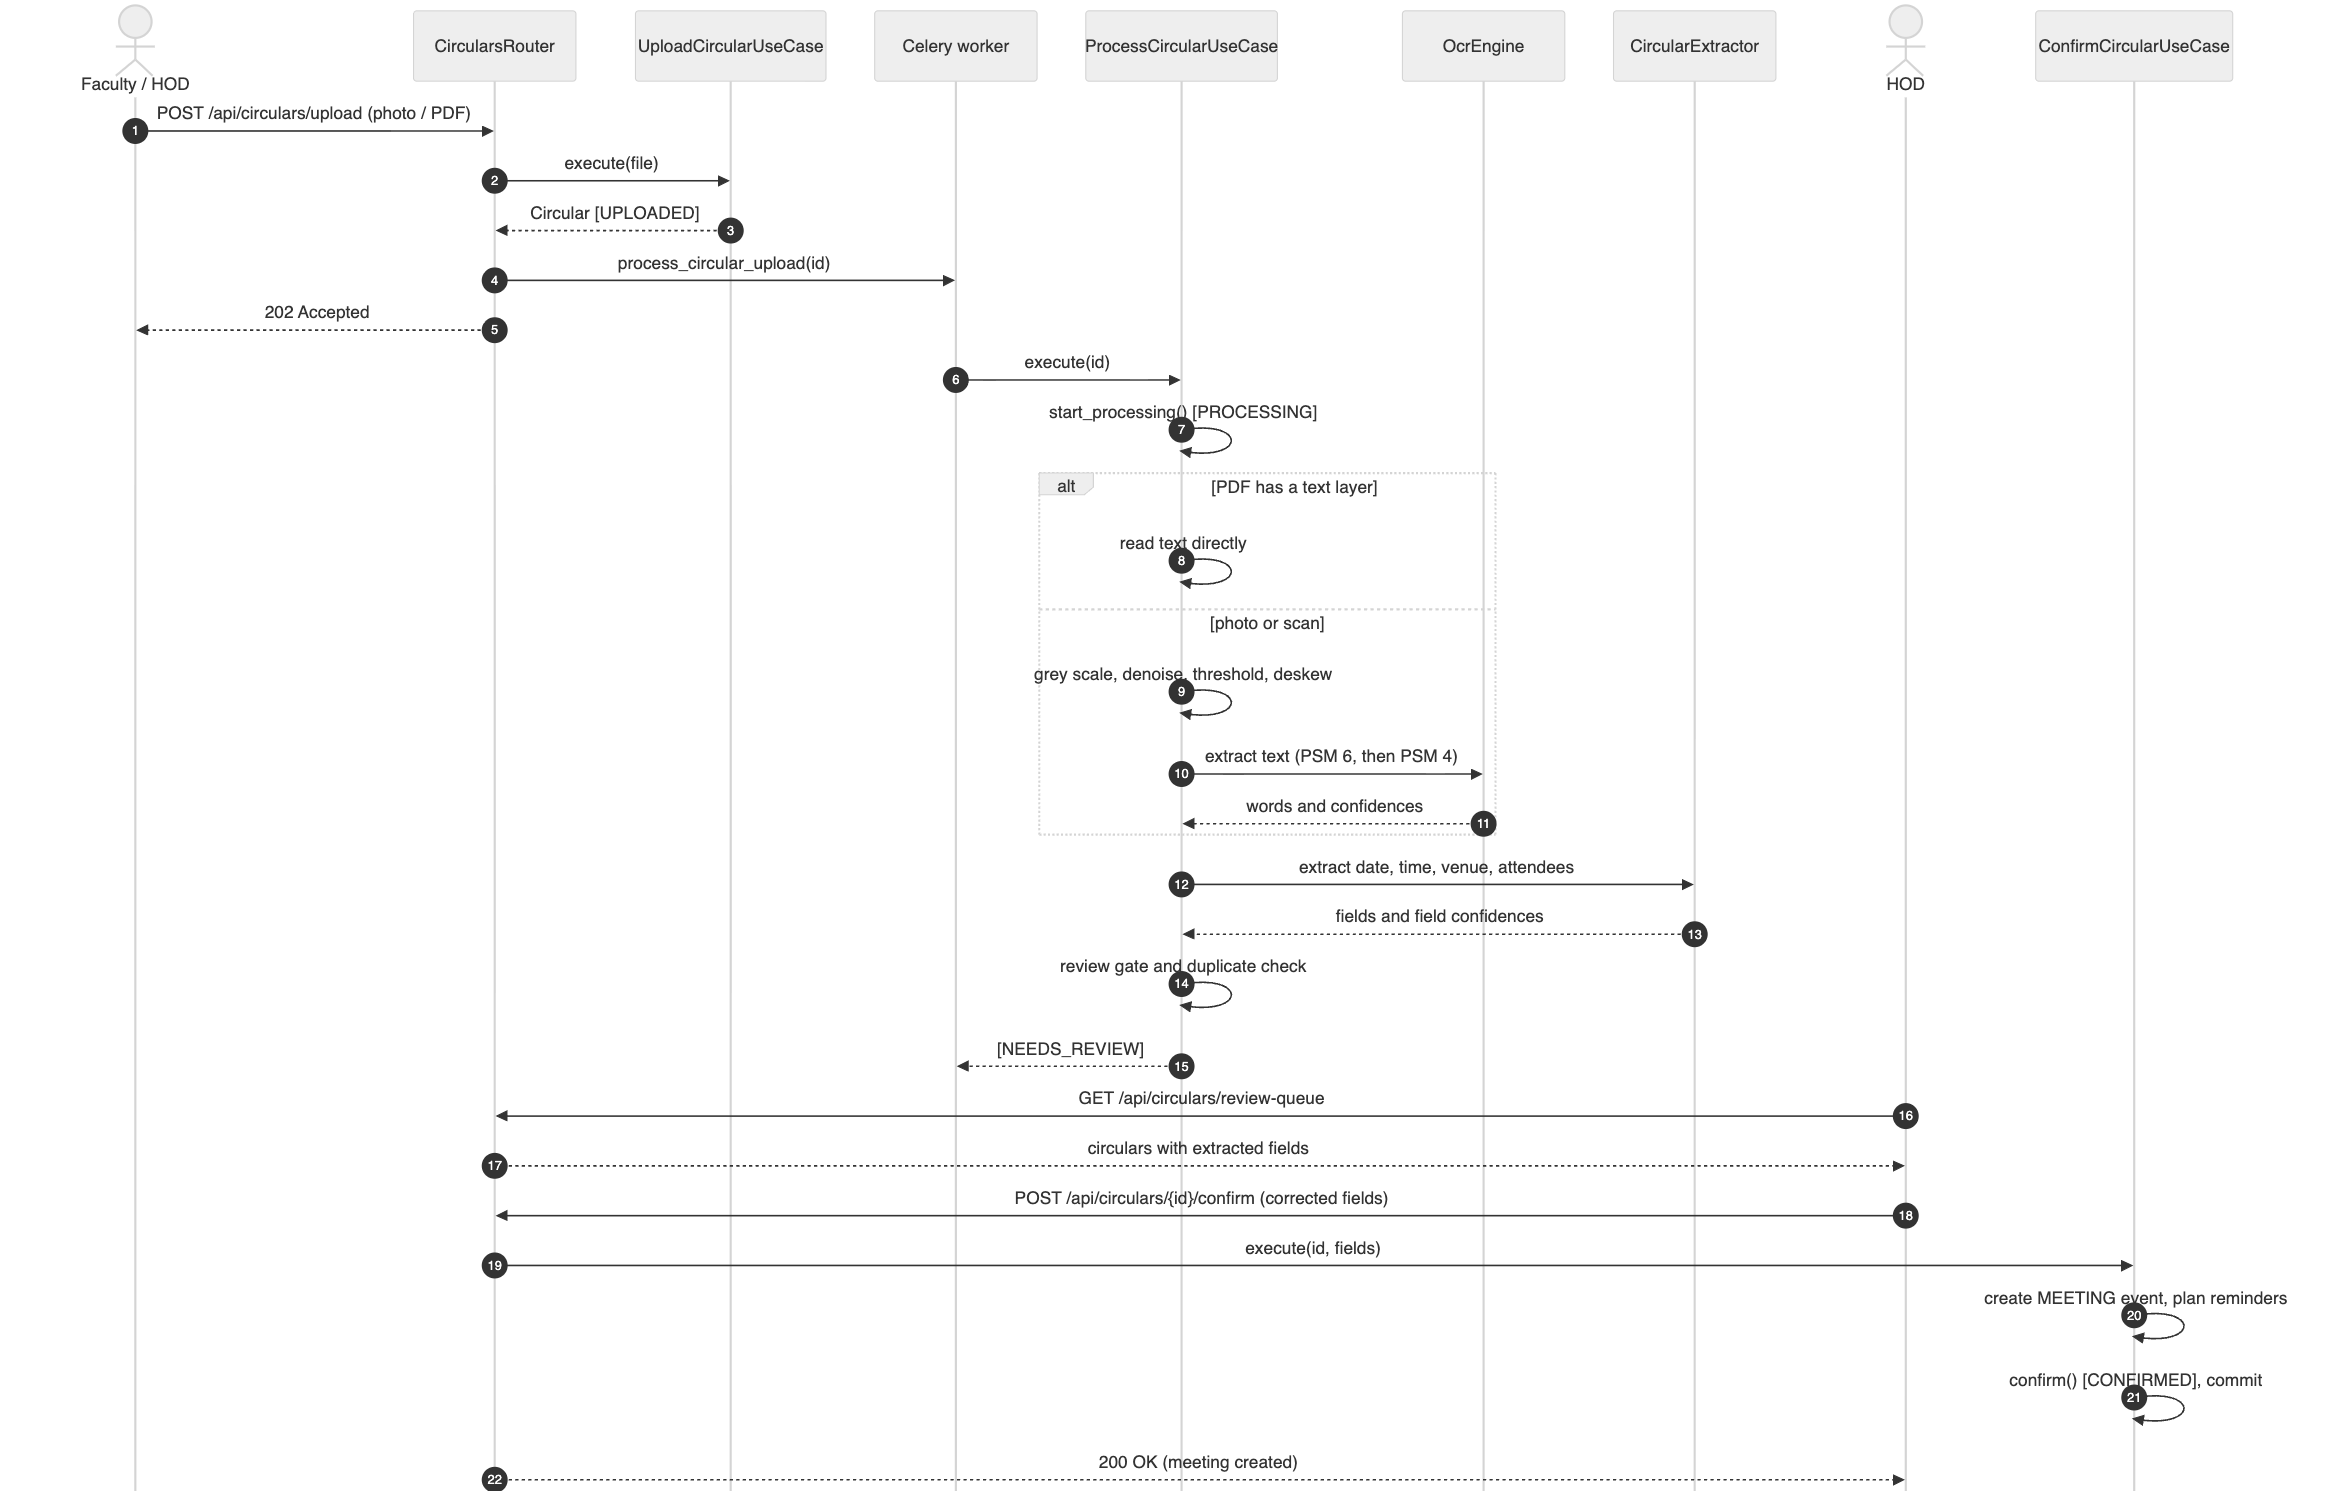
\includegraphics[width=\textwidth]{figures/seq_circular.png}
  \caption{Sequence diagram: circular upload, OCR, review and confirmation}
  \label{fig:seqcirc}
\end{figure}

\head{Explanation}
\begin{enumerate}
  \item Upload is answered immediately (1--5); processing runs in a worker (6--7).
  \item The \texttt{alt} fragment shows the two reading paths: a PDF with a text layer is read directly (8); a photo or scan is cleaned and read by \texttt{OcrEngine} with two page-segmentation modes (9--11).
  \item \texttt{CircularExtractor} returns the fields with a confidence for each (12--13), and the review gate puts the circular in NEEDS\_REVIEW (14--15).
  \item The HOD opens the review queue, corrects the fields and confirms (16--19); \texttt{ConfirmCircularUseCase} creates the meeting, plans reminders and commits (20--22).
\end{enumerate}

\begin{figure}[!htbp]
  \centering
  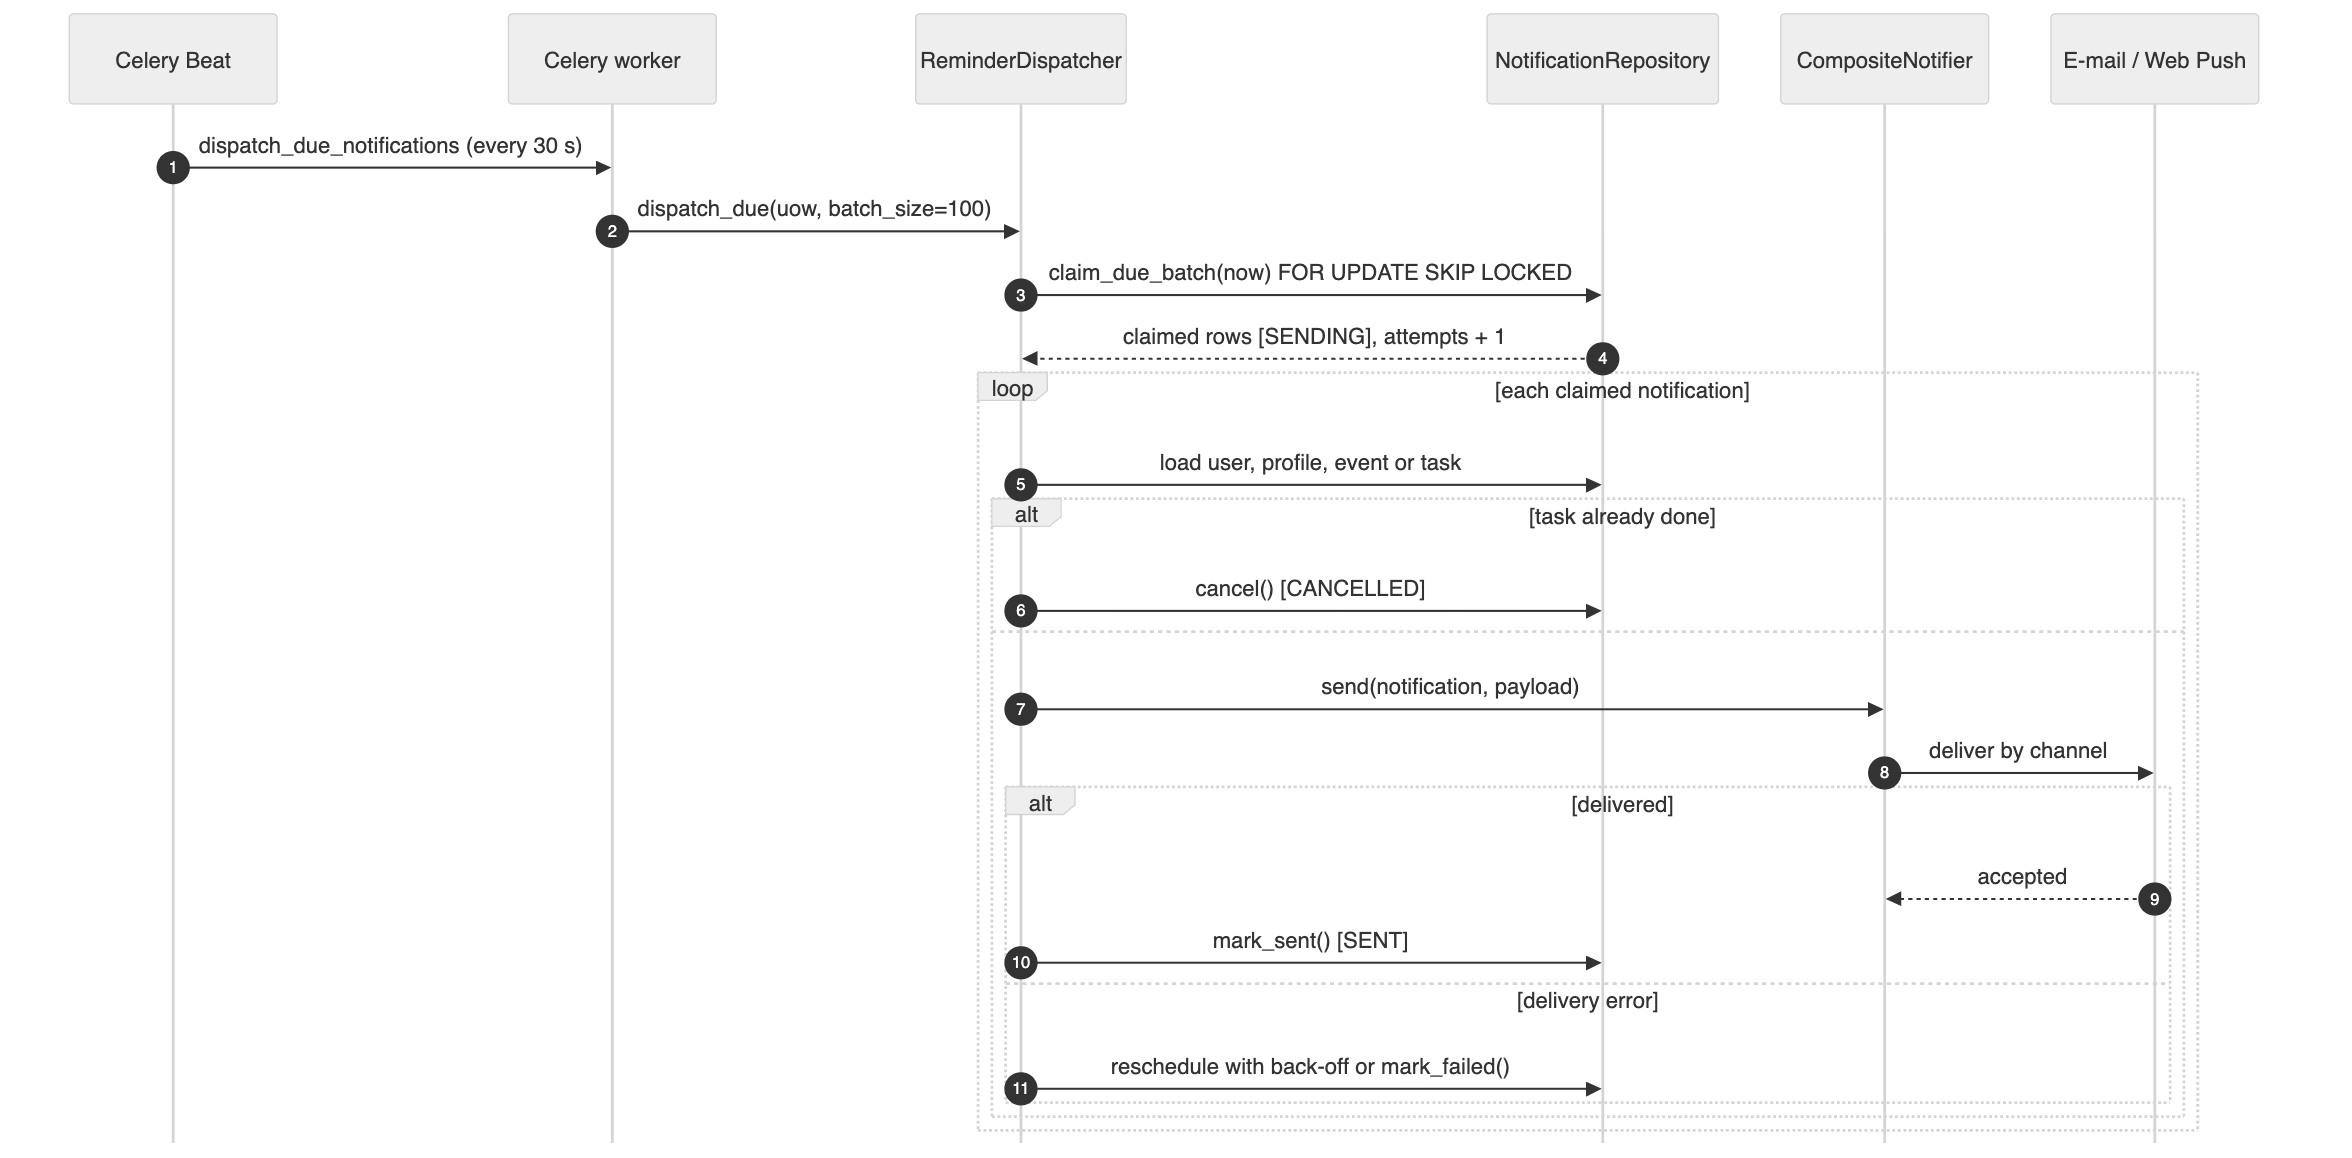
\includegraphics[width=0.95\textwidth]{figures/seq_dispatch.png}
  \caption{Sequence diagram: periodic reminder dispatch}
  \label{fig:seqdisp}
\end{figure}

\head{Explanation}
\begin{enumerate}
  \item Every 30 seconds Celery Beat starts the dispatch job (1--2).
  \item The dispatcher claims up to 100 due reminders with \texttt{SELECT ... FOR UPDATE SKIP LOCKED}, so two workers can never claim the same row, and marks them SENDING (3--4).
  \item For each reminder it loads the user and the event or task (5). If the task is already done, the reminder is cancelled; otherwise it is sent through \texttt{CompositeNotifier}, which chooses e-mail or web push (6--8).
  \item A successful send is marked SENT; a failed one is rescheduled with back-off or marked FAILED after five attempts (9--11).
\end{enumerate}

\head{Conclusion}
The three sequence diagrams show the time order of the main flows and the design decision behind them: slow work is moved to workers so that users always get an immediate answer.

\subsection{Collaboration (Communication) Diagram}

\theory{Theory}
A collaboration diagram, called a communication diagram in UML 2, shows the same interaction as a sequence diagram but arranges the objects by their links instead of by time. Messages are written along the links and numbered in nested decimal form (1, 1.1, 1.1.1), so the order and the call nesting are still visible.

\needspace{7\baselineskip}
\begin{xltabular}{\textwidth}{|p{3.2cm}|Y|Y|}
\caption{Sequence versus collaboration diagram}\\
\hline
\textbf{Point} & \textbf{Sequence diagram} & \textbf{Collaboration diagram} \\ \hline
Emphasis & Time order of messages & Structural links between objects \\ \hline
Layout & Lifelines from left to right, time downwards & Objects placed freely, joined by links \\ \hline
Message order & Vertical position & Decimal numbers (1, 1.1, 1.1.1) \\ \hline
Best for & Long flows with many steps & Seeing which objects work together \\ \hline
\end{xltabular}

\begin{figure}[!htbp]
  \centering
  \resizebox{\textwidth}{!}{\begin{tikzpicture}[
    obj/.style={rectangle, draw, semithick, fill=white, font=\footnotesize, minimum height=0.9cm, inner xsep=6pt, align=center},
    link/.style={semithick},
    msg/.style={font=\scriptsize, inner sep=2pt, align=center}
  ]
  \pic at (0,-0.4) {actor={hod : HOD}};
  \node[obj] (router) at (6.0,0) {\underline{: CircularsRouter}};
  \node[obj] (confirm) at (6.0,-3.4) {\underline{: ConfirmCircularUseCase}};
  \node[obj] (circ) at (12.6,-3.4) {\underline{circular : Circular}};
  \node[obj] (create) at (6.0,-7.2) {\underline{: CreateEventUseCase}};
  \node[obj] (uow) at (12.6,-7.2) {\underline{uow : SqlAlchemyUnitOfWork}};
  \node[obj] (clash) at (0.6,-11.2) {\underline{: CheckClashesUseCase}};
  \node[obj] (event) at (6.0,-11.2) {\underline{event : Event}};
  \node[obj] (planner) at (12.6,-11.2) {\underline{: ReminderPlanner}};

  \draw[link] (0.5,0) -- node[msg, above] {1: POST /confirm(fields) $\rightarrow$} (router);
  \draw[link] (router) -- node[msg, right] {1.1: execute(circular\_id, fields) $\downarrow$} (confirm);
  \draw[link] (confirm) -- node[msg, above] {1.1.3: confirm(fields) $\rightarrow$} (circ);
  \draw[link] (confirm.south east) -- node[msg, above right, pos=0.3] {1.1.1: circulars.get\_by\_id(id)\\1.1.4: circulars.save(circular)\\1.1.5: commit() $\searrow$} (uow.north west);
  \draw[link] (confirm) -- node[msg, left] {1.1.2: execute(MEETING, start, end,\\venue, attendees,\\override=True) $\downarrow$} (create);
  \draw[link] (create) -- node[msg, above, pos=0.4] {1.1.2.3:\\events.save(event) $\rightarrow$} (uow);
  \draw[link] (create.south west) -- node[msg, above left, pos=0.45] {1.1.2.1: execute(start, end,\\attendee\_ids) $\swarrow$} (clash.north east);
  \draw[link] (create) -- node[msg, left] {1.1.2.2: new Event(...),\\add\_attendee() $\downarrow$} (event);
  \draw[link] (create.south east) -- node[msg, below right, pos=0.45] {1.1.2.4: plan\_event\_reminders\\(event) $\searrow$} (planner.north west);
  \draw[link] (planner) -- node[msg, right] {$\uparrow$ 1.1.2.4.1:\\notifications.save(n)\\per attendee,\\offset, channel} (uow);
\end{tikzpicture}
}
  \caption{Collaboration diagram: HOD confirms a meeting circular}
  \label{fig:collab}
\end{figure}

\head{Messages}
{\small
\needspace{7\baselineskip}
\begin{xltabular}{\textwidth}{|p{1.3cm}|p{3.6cm}|p{3.6cm}|Y|}
\caption{Messages in the collaboration diagram}\\
\hline
\textbf{No.} & \textbf{From} & \textbf{To} & \textbf{Message and purpose} \\ \hline
1 & HOD & CircularsRouter & POST /confirm with the corrected fields \\ \hline
1.1 & CircularsRouter & ConfirmCircularUseCase & execute(circular\_id, fields) \\ \hline
1.1.1 & ConfirmCircularUseCase & uow (circulars) & load the circular \\ \hline
1.1.2 & ConfirmCircularUseCase & CreateEventUseCase & create a MEETING with clash override \\ \hline
1.1.2.1 & CreateEventUseCase & CheckClashesUseCase & find clashes for all attendees \\ \hline
1.1.2.2 & CreateEventUseCase & event : Event & build the event and add attendees \\ \hline
1.1.2.3 & CreateEventUseCase & uow (events) & save the event \\ \hline
1.1.2.4 & CreateEventUseCase & ReminderPlanner & plan reminders for every attendee \\ \hline
1.1.2.4.1 & ReminderPlanner & uow (notifications) & save one notification per attendee, offset, channel \\ \hline
1.1.3 & ConfirmCircularUseCase & circular : Circular & confirm(fields): status becomes CONFIRMED \\ \hline
1.1.4--1.1.5 & ConfirmCircularUseCase & uow & save the circular and commit once \\ \hline
\end{xltabular}}

\head{Conclusion}
The collaboration diagram shows that one confirmation touches eight objects, and that every write goes through the same unit of work, so the circular, the meeting, its attendees and its reminders are stored together or not at all. The clash check runs but is overridden, because the HOD has already reviewed the meeting.

\subsection{Statechart Diagrams}

\theory{Theory}
A statechart (state machine) diagram describes the states an object passes through during its life and the events that move it from one state to another. It is most useful for objects whose behaviour depends on their current state. In FacultyDesk three classes keep their allowed transitions in a table in the code and raise \texttt{InvalidTransition} for any other move.

\theory{Statechart Notation}
\needspace{7\baselineskip}
\begin{xltabular}{\textwidth}{|p{3cm}|>{\centering\arraybackslash}p{3.4cm}|Y|}
\caption{Statechart notation}\\
\hline
\textbf{Element} & \textbf{Symbol} & \textbf{Meaning} \\ \hline
Initial state & \syminit & Starting point of the object's life. \\ \hline
State & \symstate{State} & A condition in which the object waits or does work. \\ \hline
Transition & \symtrans & Change of state caused by an event. \\ \hline
Final state & \symfinal & End of the object's life. \\ \hline
\end{xltabular}

\begin{figure}[!htbp]
  \centering
  \resizebox{\textwidth}{!}{\circularstate}
  \caption{Statechart diagram of Circular}
  \label{fig:states}
\end{figure}
\needspace{7\baselineskip}
\begin{xltabular}{\textwidth}{|p{3cm}|Y|p{3.2cm}|}
\caption{State transition table: Circular}\\
\hline
\textbf{Current state} & \textbf{Event} & \textbf{Next state} \\ \hline
Initial & File stored & UPLOADED \\ \hline
UPLOADED & start\_processing() & PROCESSING \\ \hline
PROCESSING & mark\_needs\_review() (gate failed) & NEEDS\_REVIEW \\ \hline
PROCESSING & confirm() (gate passed, auto-confirm on) & CONFIRMED \\ \hline
PROCESSING & fail(reason) (file or OCR error) & FAILED \\ \hline
FAILED & start\_processing() (retry) & PROCESSING \\ \hline
NEEDS\_REVIEW & confirm() by HOD & CONFIRMED \\ \hline
NEEDS\_REVIEW & reject(reason) by HOD & REJECTED \\ \hline
\end{xltabular}

\begin{figure}[!htbp]
  \centering
  \resizebox{0.9\textwidth}{!}{\notificationstate}
  \caption{Statechart diagram of ScheduledNotification}
\end{figure}
\needspace{7\baselineskip}
\begin{xltabular}{\textwidth}{|p{3cm}|Y|p{3.2cm}|}
\caption{State transition table: ScheduledNotification}\\
\hline
\textbf{Current state} & \textbf{Event} & \textbf{Next state} \\ \hline
Initial & Reminder planned & PENDING \\ \hline
PENDING & mark\_sending() (claimed by dispatcher; attempts + 1) & SENDING \\ \hline
PENDING & cancel() (event cancelled or task done) & CANCELLED \\ \hline
SENDING & mark\_sent() & SENT \\ \hline
SENDING & mark\_failed(error) & FAILED \\ \hline
SENDING & stale recovery (more than 5 minutes) & PENDING \\ \hline
FAILED & retry() while attempts $< 5$ & PENDING \\ \hline
\end{xltabular}

\begin{figure}[!htbp]
  \centering
  \resizebox{\textwidth}{!}{\uploadstate}
  \caption{Statechart diagram of TimetableUpload}
\end{figure}
\needspace{7\baselineskip}
\begin{xltabular}{\textwidth}{|p{3.4cm}|Y|p{3.2cm}|}
\caption{State transition table: TimetableUpload}\\
\hline
\textbf{Current state} & \textbf{Event} & \textbf{Next state} \\ \hline
UPLOADED & start\_parsing() & PARSING \\ \hline
PARSING & mark\_preview\_ready(report) & PREVIEW\_READY \\ \hline
PREVIEW\_READY & confirm() by HOD & CONFIRMED \\ \hline
any non-final state & fail(reason) & FAILED \\ \hline
\end{xltabular}

\head{Conclusion}
The statecharts make the life cycle of each important object explicit. Because the same tables are enforced in code, a circular can never be confirmed twice and a reminder can never be sent from the wrong state.

\subsection{Activity Diagram}

\theory{Theory}
An activity diagram shows the flow of control from one action to the next, similar to a flowchart, with support for decisions, parallel work and swimlanes that show who performs each action. It is used to model business processes and workflows.

\theory{Activity Diagram Notation}
\needspace{7\baselineskip}
\begin{xltabular}{\textwidth}{|p{3cm}|>{\centering\arraybackslash}p{3cm}|Y|}
\caption{Activity diagram notation}\\
\hline
\textbf{Element} & \textbf{Symbol} & \textbf{Meaning} \\ \hline
Initial node & \syminit & Start of the activity. \\ \hline
Action & \symstate{Action} & A single step of work. \\ \hline
Decision / merge & \symdecision & Choose one path based on a guard, or merge paths. \\ \hline
Fork / join & \symfork & Split into, or synchronise, parallel flows. \\ \hline
Control flow & \symflow & Order in which actions execute. \\ \hline
Swimlane & -- & Partition showing who performs the actions. \\ \hline
Final node & \symfinal & End of the activity. \\ \hline
\end{xltabular}

\begin{figure}[!htbp]
  \centering
  \resizebox{!}{0.72\textheight}{\begin{tikzpicture}[
    act/.style={rectangle, rounded corners=6pt, draw, semithick, fill=actfill, text width=3.7cm, align=center, font=\footnotesize, minimum height=0.85cm},
    dec/.style={diamond, draw, semithick, fill=decfill, aspect=2.2, font=\scriptsize, inner sep=1pt, align=center},
    fl/.style={semithick, -{Stealth[length=2.2mm]}},
    g/.style={font=\scriptsize, fill=white, inner sep=1pt}
  ]
  \def\lanew{5.4}
  \foreach \i/\name in {0/HOD or Admin, 1/API server, 2/Celery worker} {
    \draw[semithick] (\i*\lanew,0.6) rectangle ++(\lanew,-23.8);
    \node[font=\bfseries\small] at (\i*\lanew+\lanew/2,0.15) {\name};
  }
  \draw[semithick] (0,-0.25) -- (3*\lanew,-0.25);

  \node[initial] (s) at (2.7,-0.9) {};
  \node[act] (sel) at (2.7,-2.0) {Choose term and timetable file (xlsx, csv, pdf)};
  \node[act] (val) at (8.1,-2.0) {Check size, magic bytes and type (UploadGuard)};
  \node[dec] (ok) at (8.1,-3.8) {valid?};
  \node[act] (rej) at (2.7,-3.8) {See rejection message};
  \node[final] (e0) at (2.7,-5.0) {};
  \node[act] (store) at (8.1,-5.8) {Store file in MinIO, save upload as UPLOADED, enqueue job};

  \node[act] (fac) at (13.5,-5.8) {Factory picks parser by sniffed MIME type};
  \node[act] (parse) at (13.5,-7.6) {Parse grid; expand merged period cells};
  \node[act] (tok) at (13.5,-9.7) {Tokenise cells into course, section, room, initials; split co-teachers};
  \node[act] (res) at (13.5,-12.0) {Resolve initials: exact, then alias, then fuzzy ($s\ge0.85$, margin $\ge0.10$)};
  \node[act] (prev) at (13.5,-14.3) {Build preview and issue report; status PREVIEW\_READY};

  \node[act] (look) at (2.7,-14.3) {Review preview and unresolved tokens};
  \node[dec] (good) at (2.7,-16.3) {issues?};
  \node[act] (fix) at (2.7,-18.3) {Fix directory aliases or file};
  \node[act] (conf) at (8.1,-16.3) {Save courses, sections, rooms, slots; status CONFIRMED};

  \node[act] (exp) at (13.5,-18.3) {Expand weekly recurrence over the term, skip holidays};
  \node[act] (ev) at (13.5,-20.2) {Create CLASS events and attendees};
  \node[act] (rem) at (13.5,-22.1) {Plan reminders with idempotency keys};
  \node[final] (e1) at (8.1,-22.1) {};

  \draw[fl] (s) -- (sel);
  \draw[fl] (sel) -- (val);
  \draw[fl] (val) -- (ok);
  \draw[fl] (ok) -- node[g, above] {[no]} (rej);
  \draw[fl] (rej) -- (e0);
  \draw[fl] (ok) -- node[g, right] {[yes]} (store);
  \draw[fl] (store) -- (fac);
  \draw[fl] (fac) -- (parse);
  \draw[fl] (parse) -- (tok);
  \draw[fl] (tok) -- (res);
  \draw[fl] (res) -- (prev);
  \draw[fl] (prev) -- (look);
  \draw[fl] (look) -- (good);
  \draw[fl] (good) -- node[g, right] {[yes]} (fix);
  \draw[fl] (fix.west) -- ++(-0.35,0) |- (sel.west);
  \draw[fl] (good) -- node[g, above] {[no]} (conf);
  \draw[fl] (conf.east) -| (exp.north);
  \draw[fl] (exp) -- (ev);
  \draw[fl] (ev) -- (rem);
  \draw[fl] (rem) -- (e1);
\end{tikzpicture}
}
  \caption{Activity diagram: timetable ingestion and initials resolution}
  \label{fig:activity}
\end{figure}

\head{Explanation}
\begin{itemize}
  \item \textbf{Swimlanes:} the HOD, the API server and the Celery worker each perform their own actions.
  \item \textbf{First decision:} an invalid file is rejected before anything is stored.
  \item \textbf{Worker steps:} the factory chooses the parser; cells are split into course, section, room and initials; co-teacher cells are split; initials are resolved in three tiers.
  \item \textbf{Second decision and loop:} if the preview shows issues, the HOD fixes aliases or the file and uploads again; only a clean preview is confirmed.
  \item \textbf{After confirmation:} weekly recurrence is expanded over the term, holidays are skipped, CLASS events are created and reminders are planned.
\end{itemize}

\head{Activities Identified}
\needspace{7\baselineskip}
\begin{xltabular}{\textwidth}{|p{1cm}|Y|p{2.6cm}|p{3cm}|}
\caption{Activities in timetable ingestion}\\
\hline
\textbf{No.} & \textbf{Activity} & \textbf{Swimlane} & \textbf{Type} \\ \hline
1 & Choose term and timetable file & HOD & Action \\ \hline
2 & Check size, file type and content & API server & Action + decision \\ \hline
3 & Store file and enqueue the job & API server & Action \\ \hline
4 & Pick parser and parse the grid & Worker & Action \\ \hline
5 & Tokenise cells and split co-teachers & Worker & Action \\ \hline
6 & Resolve initials (exact, alias, fuzzy) & Worker & Action \\ \hline
7 & Build preview and issue report & Worker & Action \\ \hline
8 & Review preview; fix issues if any & HOD & Decision (loop to 1) \\ \hline
9 & Save courses, sections, rooms, slots & API server & Action \\ \hline
10 & Expand recurrence, create events, plan reminders & Worker & Action \\ \hline
\end{xltabular}

\head{Conclusion}
The activity diagram models the complete ingestion workflow, including the validation stop, the fix-and-retry loop and the division of work between the HOD, the API and the background worker.

\subsection{Package Diagram}

\theory{Theory}
A package diagram groups model elements or code into packages and shows the dependencies between them. A package is drawn as a folder (\sympkg); a dependency is a dashed arrow, often labelled \guill{import} or \guill{use}. It is used to check that the layering of a system is respected.

\begin{figure}[!htbp]
  \centering
  \resizebox{0.95\textwidth}{!}{\begin{tikzpicture}[
    pkg/.style={rectangle, draw, semithick, fill=#1, align=left, font=\scriptsize\sffamily, inner sep=5pt, text width=3.6cm, minimum height=1.6cm},
    pkg/.default=white,
    tab/.style={draw, semithick, fill=white, font=\footnotesize\bfseries, inner sep=2.5pt, anchor=south west},
    imp/.style={semithick, dashed, -{Stealth[length=2.4mm]}},
    bad/.style={semithick, dashed, black, -{Stealth[length=2.4mm]}},
    lbl/.style={font=\scriptsize\itshape, fill=white, inner sep=1pt}
  ]
  \newcommand{\pkgnode}[5]{\node[pkg=#4] (#1) at (#2) {#5}; \node[tab] at (#1.north west) {#3};}

  \pkgnode{fe}{7.0,4.2}{frontend}{white}{app/ (pages)\\components/\\lib/ (api-client, auth, openapi types)}

  \pkgnode{api}{2.6,0}{api}{white}{routers/ (auth, calendar,\\ circulars, tasks, timetable,\\ directory, reminders, metrics)\\deps.py (wiring)}
  \pkgnode{workers}{11.4,0}{workers}{white}{celery\_app.py\\timetable\_tasks, circular\_tasks,\\reminder\_tasks, task\_alerts,\\calendar\_tasks, backup\_tasks}

  \pkgnode{app}{7.0,-4.4}{application}{white}{auth/ directory/ timetable/\\circulars/ calendar/\\reminders/ tasks/ security/}

  \pkgnode{infra}{12.6,-8.6}{infrastructure}{white}{db/ (models, repositories, UoW)\\parsers/ ocr/ notifiers/\\storage/ security/ seed/}

  \pkgnode{dom}{7.0,-8.6}{domain}{white}{entities.py\\value\_objects.py\\events.py  errors.py\\repositories.py (interfaces)}

  \pkgnode{core}{1.4,-8.6}{core}{white}{clock.py  config.py\\db.py  redis.py  logging.py\\security.py  upload\_guard.py}

  \draw[imp] (fe.south) -- node[lbl, pos=0.4] {\guill{REST / OpenAPI}} (api.north);
  \draw[imp] (api.south) -- node[lbl, sloped] {\guill{use}} (app.north west);
  \draw[imp] (workers.south) -- node[lbl, sloped] {\guill{use}} (app.north east);
  \draw[imp] (app) -- node[lbl] {\guill{use}} (dom);
  \draw[imp] (infra) -- node[lbl] {\guill{implements}} (dom);
  \draw[imp] (workers.south east) -- node[lbl, sloped] {\guill{wires}} (infra.north);
  \draw[imp] (app.south west) -- node[lbl, sloped] {\guill{use}} (core.north east);
  \draw[imp] (api.south) ++(-1.0,0) -- node[lbl] {\guill{use}} ([xshift=0.2cm]core.north);
  \draw[bad] (app.east) -| node[lbl, pos=0.7, right, text=black, align=left] {direct import\\in 4 files} ([xshift=-1.2cm]infra.north);
\end{tikzpicture}
}
  \caption{Package diagram with import dependencies}
  \label{fig:package}
\end{figure}

\head{Explanation}
\begin{itemize}
  \item The \textbf{frontend} calls the backend only through the REST API described by an OpenAPI contract.
  \item \textbf{api} and \textbf{workers} call \textbf{application}; \textbf{workers} (and \texttt{api/deps.py}) wire the concrete adapters from \textbf{infrastructure}.
  \item \textbf{infrastructure} implements the repository interfaces declared in \textbf{domain}.
  \item \textbf{domain} imports nothing outside itself; we checked this by scanning every import in the backend.
  \item The arrow labelled \emph{direct import} marks four application files that import infrastructure classes (OCR engine and extractor, parser factory and initials resolver, notifier base class, MinIO storage). Moving these behind domain interfaces would complete the layering.
\end{itemize}

\head{Conclusion}
The package diagram confirms that the business core (\texttt{domain}) is independent of frameworks and shows the one place where the layering is not yet complete.

\subsection{Component Diagram}

\theory{Theory}
A component diagram shows the replaceable parts of a running system and the interfaces through which they connect. A component (\symcompnt) provides interfaces, drawn as a ball (\symball), and requires interfaces from other components.

\begin{figure}[!htbp]
  \centering
  \resizebox{\textwidth}{!}{\begin{tikzpicture}[
    comp/.style={rectangle, draw, semithick, fill=#1, align=center, font=\footnotesize, minimum width=3.6cm, minimum height=1.25cm, inner sep=4pt},
    comp/.default=white,
    ext/.style={rectangle, draw, semithick, dashed, fill=white, align=center, font=\footnotesize, minimum width=2.9cm, minimum height=1.0cm},
    con/.style={semithick, -{Stealth[length=2.2mm]}},
    ball/.style={circle, draw, semithick, fill=white, minimum size=2.6mm, inner sep=0pt},
    ilbl/.style={font=\scriptsize\itshape, inner sep=1.5pt, align=center}
  ]
  \newcommand{\cname}[2]{{\scriptsize\guill{component}}\\\textbf{#1}\\{\scriptsize #2}}

  \node[comp=white] (fe) at (0,0) {\cname{Web client}{Next.js PWA, service worker}};
  \node[comp=white] (api) at (6.4,0) {\cname{API}{FastAPI routers, AuthorisationPolicy}};
  \node[comp=white] (worker) at (12.8,0) {\cname{Worker}{Celery tasks}};
  \node[comp=white] (beat) at (12.8,3.0) {\cname{Scheduler}{Celery Beat}};
  \node[comp=white] (uc) at (9.6,-3.4) {\cname{Use cases}{application layer}};
  \node[comp=white] (dom) at (9.6,-6.6) {\cname{Domain model}{entities, value objects, interfaces}};

  \node[comp=white] (persist) at (0,-9.8) {\cname{Persistence}{SqlAlchemyUnitOfWork}};
  \node[comp=white] (store) at (4.8,-9.8) {\cname{Object storage}{MinioStorageService}};
  \node[comp=white] (ocr) at (9.6,-9.8) {\cname{OCR and parsing}{OcrEngine, parsers}};
  \node[comp=white] (notify) at (14.4,-9.8) {\cname{Notifications}{CompositeNotifier}};

  \node[ext] (pg) at (0,-12.6) {PostgreSQL 16};
  \node[ext] (minio) at (4.8,-12.6) {MinIO};
  \node[ext] (tess) at (9.6,-12.6) {Tesseract};
  \node[ext] (smtp) at (14.4,-12.6) {SMTP / Web Push\\services};
  \node[ext] (redis) at (19.0,0) {Redis 7};
  \node[ext] (cal) at (0,3.0) {External calendar\\(Google, Apple)};

  \node[ball] (restball) at (3.2,0) {};
  \node[ilbl, above] at (restball.north) {REST API};
  \draw[semithick] (api.west) -- (restball);
  \draw[con] (fe.east) -- (restball.west);
  \node[ball] (icsball) at (6.4,3.0) {};
  \node[ilbl, above] at (icsball.north) {ICS feed};
  \draw[semithick] (api.north) -- (icsball);
  \draw[con] (cal.east) -- (icsball.west);

  \draw[con] (api.south) |- node[ilbl, pos=0.25, left] {calls} (uc.west);
  \draw[con] (worker.south) |- node[ilbl, pos=0.25, right] {calls} (uc.east);
  \draw[con] (beat) -- node[ilbl, right] {schedules} (worker);
  \draw[con] (api.east) -- node[ilbl, above] {enqueue} (worker.west);
  \draw[con] (worker.east) -- (redis.west);
  \draw[con] (uc) -- (dom);

  \foreach \c/\i in {persist/UnitOfWork, store/StorageService, ocr/OcrEngine, notify/Notifier} {
    \node[ball] (\c b) at ($(\c.north)+(0,0.75)$) {};
    \node[ilbl, right] at (\c b.east) {\i};
    \draw[semithick] (\c.north) -- (\c b);
  }
  \draw[con] (dom.south west) -- ++(0,-0.5) -| (persistb.north);
  \draw[con] (uc.south west) -- ++(-0.4,-0.5) -| (storeb.north);
  \draw[con] (uc.south east) -- ++(1.2,-0.5) -| (notifyb.north);
  \draw[con] ([yshift=-3mm]uc.east) -- (13.0,-3.7) -- (13.0,-8.0) -| (ocrb.north);

  \draw[con] (persist) -- (pg);
  \draw[con] (store) -- (minio);
  \draw[con] (ocr) -- (tess);
  \draw[con] (notify) -- (smtp);
\end{tikzpicture}
}
  \caption{Component diagram with provided interfaces}
  \label{fig:component}
\end{figure}

\head{Components Identified}
{\small
\needspace{7\baselineskip}
\begin{xltabular}{\textwidth}{|p{3.2cm}|Y|p{4.2cm}|}
\caption{Components and interfaces}\\
\hline
\textbf{Component} & \textbf{Responsibility} & \textbf{Interface} \\ \hline
Web client & Screens for all roles; offline cache and push handler & requires REST API \\ \hline
API & Routers, validation, role checks & provides REST API, ICS feed \\ \hline
Worker / Scheduler & Background jobs and periodic schedule & uses Redis queue \\ \hline
Use cases & One class per user goal & requires UnitOfWork, StorageService, OcrEngine, Notifier \\ \hline
Domain model & Entities, value objects, interfaces & declares repository interfaces \\ \hline
Persistence & SQLAlchemy repositories and unit of work & provides UnitOfWork \\ \hline
Object storage & File upload and download in MinIO & provides StorageService \\ \hline
OCR and parsing & Tesseract OCR, timetable parsers & provides OcrEngine \\ \hline
Notifications & E-mail and web push & provides Notifier \\ \hline
\end{xltabular}}

\head{Conclusion}
The component diagram shows that the API and the worker share the same use-case component, and that every external service is reached through one adapter, so it can be replaced without changing the use cases. \texttt{UnitOfWork} and \texttt{Notifier} are abstract types in the code; \texttt{OcrEngine} and \texttt{StorageService} are concrete classes today.

\subsection{Deployment Diagram}

\theory{Theory}
A deployment diagram shows the physical nodes (devices and execution environments, drawn as 3-D boxes \symnode), the artifacts deployed on them, and the communication paths between nodes.

\begin{figure}[!htbp]
  \centering
  \resizebox{\textwidth}{!}{\begin{tikzpicture}[
    art/.style={rectangle, draw, semithick, fill=white, font=\scriptsize, align=center, minimum width=2.9cm, minimum height=0.95cm},
    path/.style={semithick},
    l/.style={font=\scriptsize\itshape, fill=white, inner sep=1pt, align=center}
  ]
  \newcommand{\umlnode}[5]{%
    \draw[semithick, fill=white] (#1) rectangle ++(#2,-#3);
    \draw[semithick] (#1) -- ++(0.3,0.3) -- ++(#2,0) -- ++(0,-#3) -- ++(-0.3,-0.3);
    \draw[semithick] ($(#1)+(#2,0)$) -- ++(0.3,0.3);
    \node[anchor=north west, font=\scriptsize, align=left, fill=white, inner sep=1pt] at ($(#1)+(0.1,-0.08)$) {\guill{#4}\\\textbf{#5}};}

  \umlnode{0,0}{4.2}{3.0}{device}{Faculty phone / PC}
  \node[art] at (2.1,-1.9) {\guill{artifact}\\Browser / installed PWA};

  \umlnode{0,-4.2}{4.2}{2.8}{device}{External calendar client}
  \node[art] at (2.1,-5.95) {Google / Apple Calendar};

  \umlnode{5.6,1.2}{10.6}{11.8}{device}{Department server (Linux, Docker Engine)}
  \node[art] (caddy) at (8.0,-1.2) {\guill{container}\\caddy : reverse proxy};
  \node[art] (fe) at (11.4,-1.2) {\guill{container}\\frontend : Next.js};
  \node[art] (be) at (14.6,-1.2) {\guill{container}\\backend : FastAPI};
  \node[art] (wk) at (11.4,-4.0) {\guill{container}\\worker : Celery};
  \node[art] (bt) at (8.0,-4.0) {\guill{container}\\beat : Celery Beat};
  \node[art] (pg) at (14.6,-4.0) {\guill{container}\\postgres : PostgreSQL 16};
  \node[art] (rd) at (8.0,-6.8) {\guill{container}\\redis : Redis 7};
  \node[art] (mn) at (14.6,-6.8) {\guill{container}\\minio : object storage};
  \node[art] (mp) at (11.4,-8.8) {\guill{container}\\mailpit (development only)};

  \umlnode{0,-8.0}{4.2}{2.8}{external}{SMTP relay / Push service}
  \node[art] (ext) at (2.1,-9.75) {E-mail and Web Push delivery};

  \draw[path] (4.2,-1.05) -- node[l, above, pos=0.35] {HTTPS 443} ([yshift=1.5mm]caddy.west);
  \draw[path] (4.2,-5.6) -- node[l, below, pos=0.5] {HTTPS (ICS)} (5.05,-5.6) -- (5.05,-1.35) -- ([yshift=-1.5mm]caddy.west);
  \draw[path] (caddy) -- (fe);
  \draw[path] (fe) -- (be);
  \draw[path] (caddy.south) -- (8.0,-2.4) -| node[l, pos=0.25, below] {/api} (be.south);
  \draw[path] (be) -- (pg);
  \draw[path] (be.east) -- ++(0.35,0) |- (mn.east);
  \draw[path] (wk) -- (pg);
  \draw[path] (wk) -- (rd);
  \draw[path] (wk) -- (mn);
  \draw[path] (bt) -- (rd);
  \draw[path] (be) -- node[l, sloped, above] {enqueue} (wk);
  \draw[path] (wk) -- (mp);
  \draw[path] (ext.east) -- node[l, above, pos=0.25] {SMTP / HTTPS} (9.7,-9.75) -- (9.7,-4.0) -- (wk.west);
\end{tikzpicture}
}
  \caption{Deployment diagram (production on a department server)}
  \label{fig:deployment}
\end{figure}

\head{Explanation}
\begin{itemize}
  \item All server parts run as containers on one machine under Docker Compose; application containers run as a non-root user.
  \item Browsers, the installed phone app and external calendar apps reach only the Caddy container over HTTPS. Caddy sends \texttt{/api} requests to the backend and all other requests to the frontend.
  \item The worker and the scheduler share PostgreSQL, Redis and MinIO with the backend; the worker delivers e-mail and web push to outside services.
  \item In \emph{college-LAN mode} Caddy uses an internal certificate, so the system can run inside the campus network without a public domain.
\end{itemize}

\head{Conclusion}
The deployment diagram shows that the complete system fits on one department server and needs no paid service.

\subsection{Entity--Relationship Diagram}
The ER diagram in Figure~\ref{fig:er} is generated by a script directly from the database model definitions, so its 20 tables, columns and keys match the database exactly. All timestamps are stored as \texttt{timestamptz} in UTC. Unique keys enforce business rules in the database itself, for example one \texttt{idempotency\_key} per reminder and one \texttt{ics\_token} per faculty member. Because the schema is wide, the diagram is rotated on the page.

\begin{figure}[H]
  \centering
  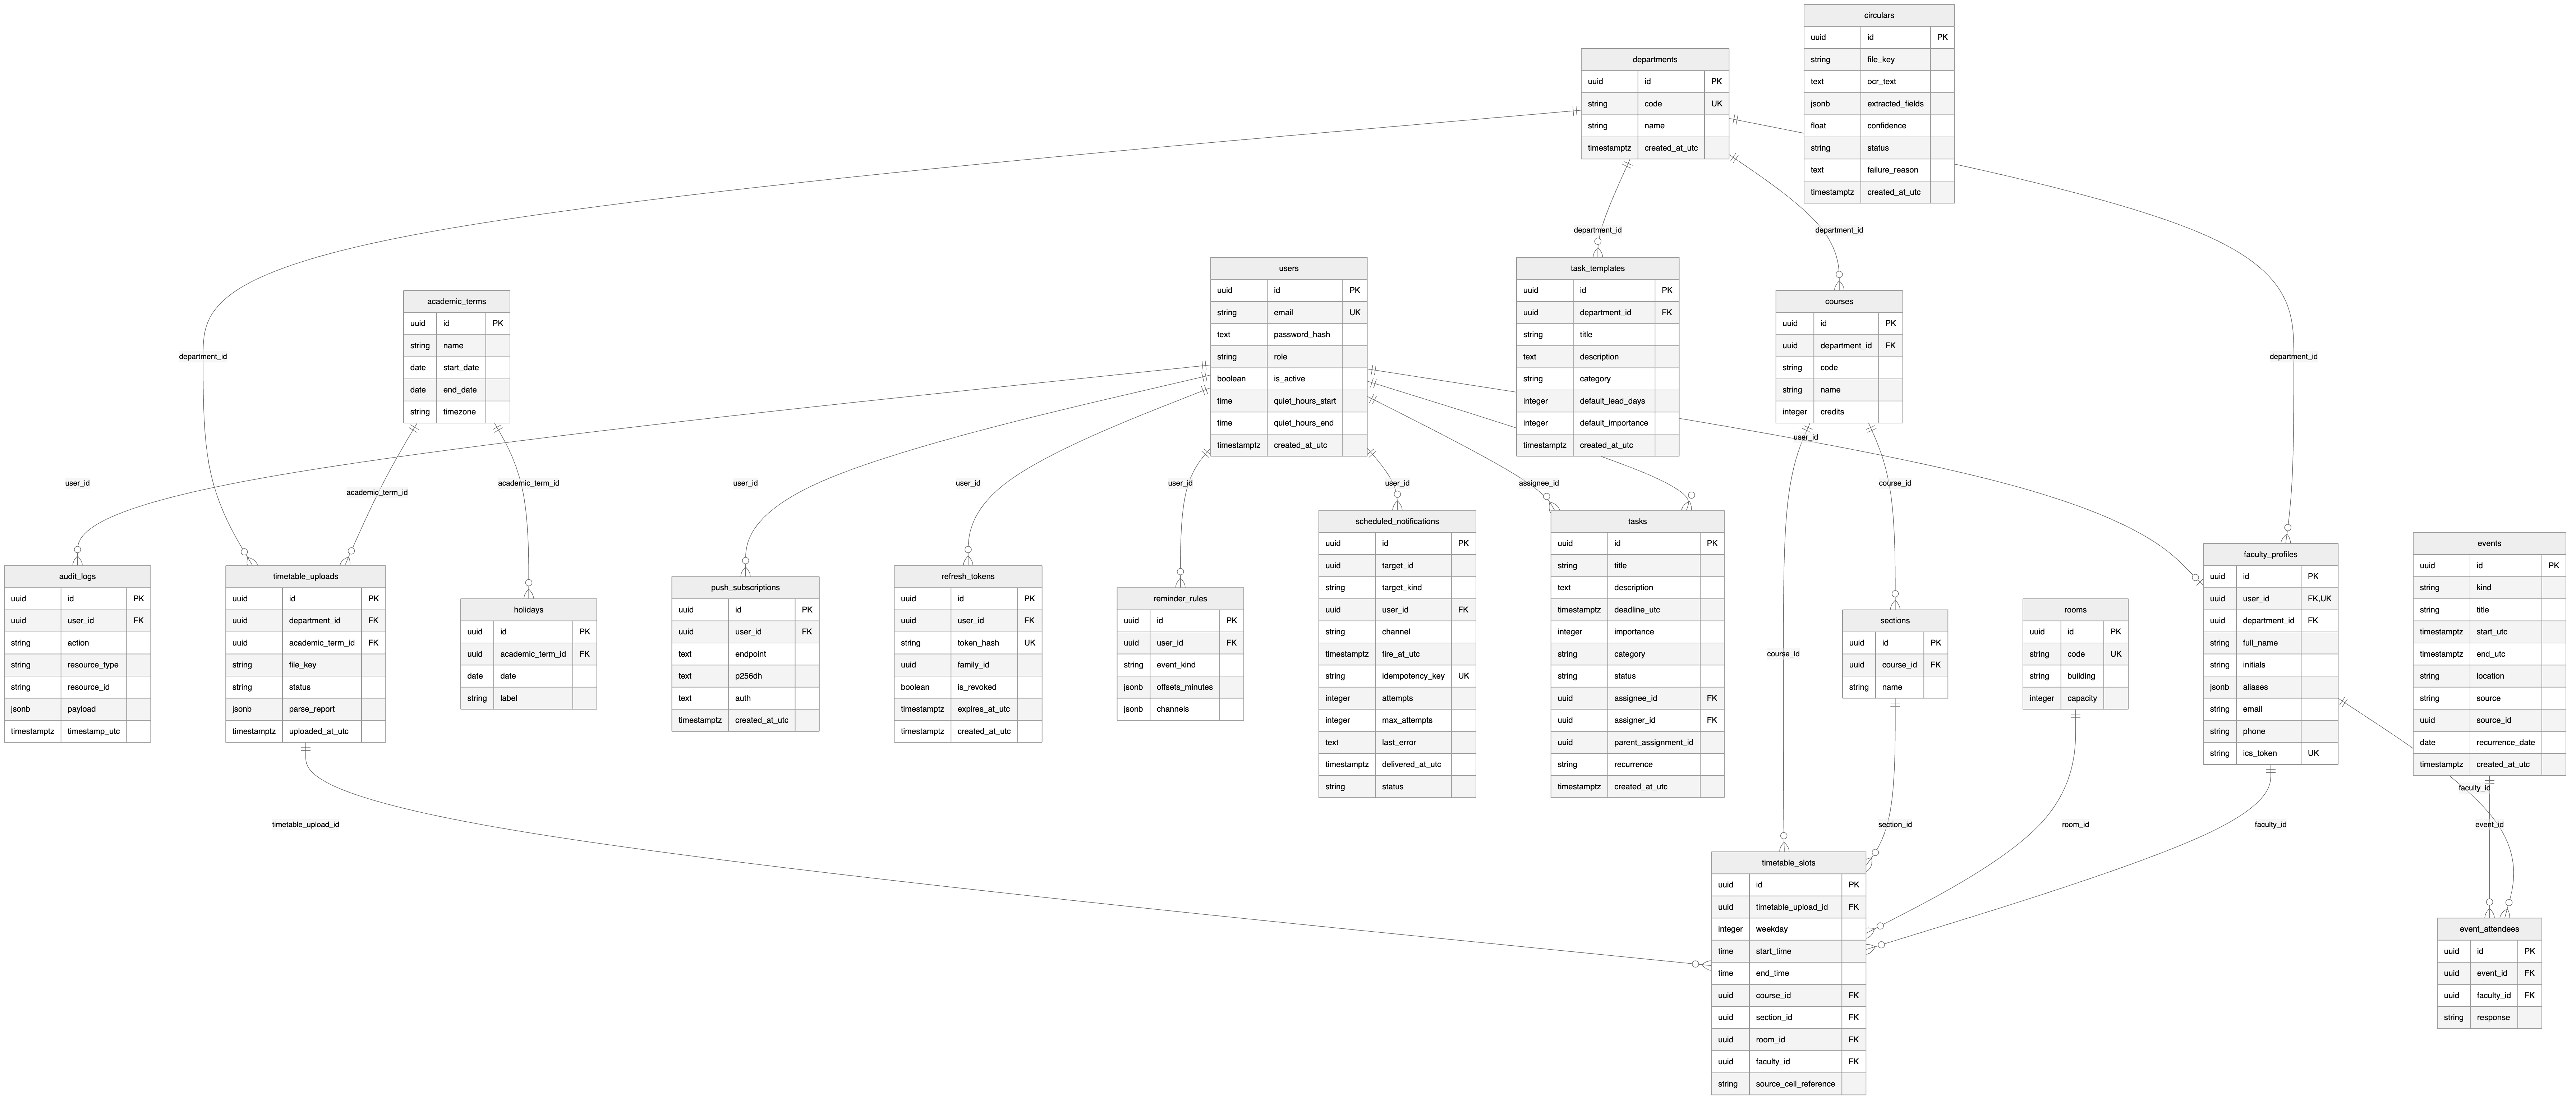
\includegraphics[angle=90, height=0.74\textheight, width=\textwidth, keepaspectratio]{figures/er-generated.png}
  \caption{Entity--relationship diagram of the PostgreSQL schema}
  \label{fig:er}
\end{figure}
